\documentclass[10pt]{article}

\usepackage[left=0.8in,right=0.8in,top=0.15in,bottom=0.8in]{geometry}
\usepackage{xcolor}
\usepackage{hyperref}
\usepackage{graphicx}
\usepackage{subfig}

\hypersetup{colorlinks=true,linkcolor=blue,urlcolor=blue}
\urlstyle{rm}
\usepackage{url}


\title{Deepfake Detection\\} 
	
\author{
        C.J. Annunziato \\
        c.annunziato@ufl.edu\\
        \and
        Edward Guthrie \\
        edwardguthrie@ufl.edu\\
        \and
        Michael Pangas \\
        mpangas@ufl.edu\\
        \and
        Parker Hovis \\
        p.hovis@ufl.edu\\
        \and
        Aaron Shumer \\
        shumera@ufl.edu\\
}


% set the date to today
\date{\today}


\begin{document} % start document tag

\maketitle


%%% Remember: writing counts! (try to be clear and concise.)
%%% Make sure to cite your sources and references (use refs.bib and \cite{} or \footnote{} for URLs).
%%%


%% TODO: write an introduction to make the report self-contained
%% Must address:
%% - What is the project about?
%%
\section{Introduction}


% TODO:
\quad Deepfakes, images of human faces which are generated by machine learning models, have rapidly become a concern of public interest due to their negative impact on the reliability of information available online~\cite{fallis2021epistemic}. A large portion of this impact is due to the highly realistic nature of deepfakes that are being generated today, with a study by Doss et al. (2023) finding that 27–50\%~\cite{doss2023deepfakes} of individuals are unable to distinguish real videos from deepfakes. Our project, Deepfake Detection using Convolutional Neural Networks, aims to employ a Convolutional Neural Network, or CNN, to prevent this existential threat~\cite{fallis2021epistemic} by exploring the effectiveness of CNNs when distinguishing between real images and deepfakes via binary classification. 


%% TODO: write about your approach / ML pipeline
%% Must contain:
%% - How you are trying to solve this problem
%% - What is the task, dataset, approach (ML techniques)?
%%
\section{Approach: Dataset(s) \& Pipeline(s)}

\quad We utilize the DeepFakeFace ~\cite{song2023robustness}dataset, an open-source collection of 120,000 images, comprised of 30,000 real images and 90,000 images generated by three distinct Stable Diffusion models. We believe DeepFakeFace's large volume and diverse representation of image generation techniques will enhance our model's ability to generalize across different sources of deepfakes, making it a better choice for training compared to datasets using only one diffusion model. This generalization is crucial for our models' usefulness outside the scope of this project, as deepfakes images encountered online may originate from varied sources and machine learning techniques.

\begin{figure}[htb!]%
    \centering
    \subfloat[\centering Model summary]{{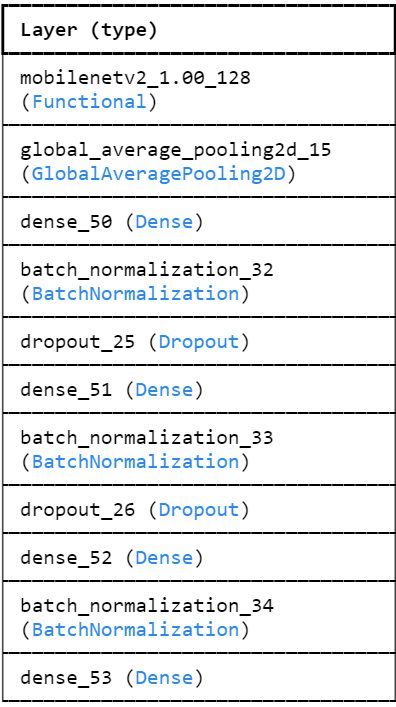
\includegraphics[width=4cm]{model.png} }}%
    \qquad
    \subfloat[\centering Example images]{{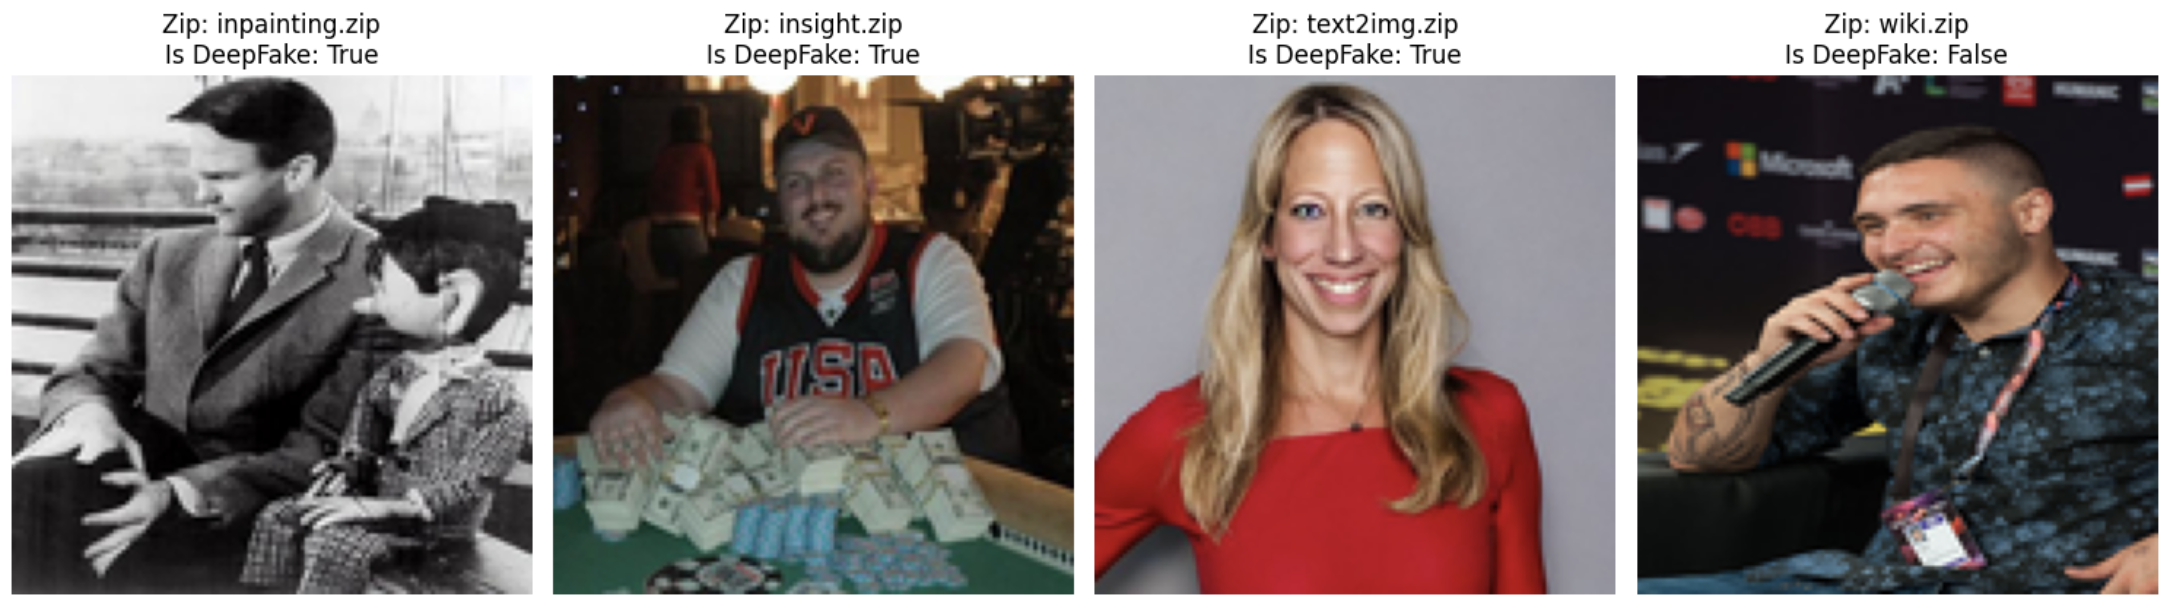
\includegraphics[width=12cm]{DataSetExample.png} }}%
    \caption{Model summary (left) Example images pulled from the dataset (right)}%
    \label{fig:example}%
\end{figure}

We opted for a Convolutional Neural Network (CNN) to differentiate between real and generated facial images due to its adeptness at extracting and learning significant features from images for classification. We applied transfer learning to MobileNetV2 by removing its top layer and adding a few more layers to the architecture (see Figure 1a). Since MobileNetV2 has been trained on millions of images, it serves as a solid base that improves our model’s ability to generalize from less data. 

The data pipeline retrieves images from the four zip archives in the dataset, designating images from wiki.zip as real and all others as deepfakes, and standardizes them for analysis. To manage training time while utilizing a significant amount of data, we decided to use only 2,000 images from each of the three diffusion model and 6,000 real images. These images are resized to 128x128 pixels, transformed to RGB color space, and flattened into a DataFrame for easy visualization. They are then restructured into a NumPy array suitable for training the CNN, with labels assigned accordingly. 







%% TODO: write about your evaluation methodology
%% Must contain:
%% - What are the metrics?
%% - What are the baselines?
%% - How did you split the data?
%%
\section{Evaluation Methodology}

% TODO:
\quad We evaluated the effectiveness of our model in performing binary classification of deepfake and real images using \textbf{Accuracy} and \textbf{$F_{1}$ Score}. 

Our first baseline for evaluating our ML pipeline is Reconstruction-Classification Learning framework (RECCE)~\cite{Cao_2022_CVPR}. RECCE is an implementation of end-to-end Reconstruction-Classification learning for face forgery detection. It has an accuracy of 0.3814, 0.5135, and 0.5899 for the Stable Diffusion v1.5, Stable Diffusion Inpainting, and Insight models, respectively. 
Our second baseline is random guessing. Randomly guessing if an image is a deepfake would have an accuracy of 0.5.

We first shuffled the data to randomize the order, then decided to split it using an 80-10-10 ratio. To ensure that half of the images in the training, test, and validation sets were fake and half were real, we used stratified sampling during the split process.

 




%% TODO: write about your results/findings
%% Must contain:
%% - results comparing your approach to baseline according to metrics
%%
%% You can present this information in whatever way you want but consider tables and (or) figures.
%%
\section{Results}
As seen in Table 1, our model proved to be better than random guessing and performed better in every metric than the RECCE model. We attained our results by testing our model on 200 images from each diffusion model. 

\begin{table}[h]
\centering
\begin{tabular}{|l|c|c|}
\hline
\textbf{Dataset}                & \textbf{Our Model}& \textbf{RECCE }\\ \hline
Stable Diffusion v1.5           & \textit{0.89}& 0.3814             \\ \hline
Stable Diffusion Inpainting     & \textit{0.7975}& 0.5135             \\ \hline
Insight& \textit{0.6925}& \textit{.5899}\\ \hline
\end{tabular}
\caption{Accuracy Comparison of Our Model and RECCE on Stable Diffusion Datasets}
\label{tab:accuracy_comparison}
\end{table}
On the test dataset, our model achieved a F1 score of .8125. Figure 3 demonstrates the correct and incorrect predictions of our model and Figure 4 shows our model's learning curve.
\begin{figure}[htb!]
    \centering
    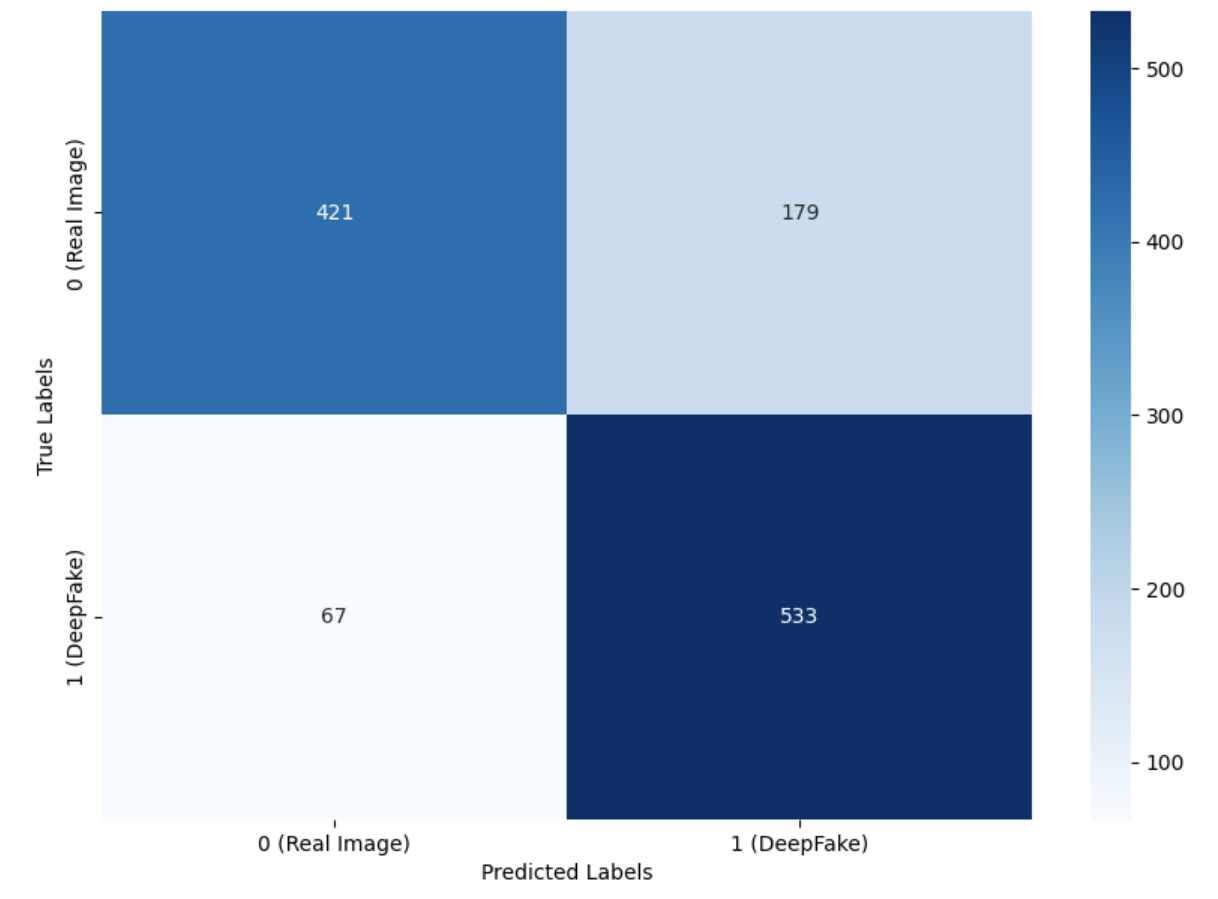
\includegraphics[width=0.5\linewidth]{confusionMatrix.png}
    \caption{Confusion matrix from the results of the our model's prediction on the test data.}
    \label{fig:fig3}
\end{figure}

\begin{figure}[htb!]
    \centering
    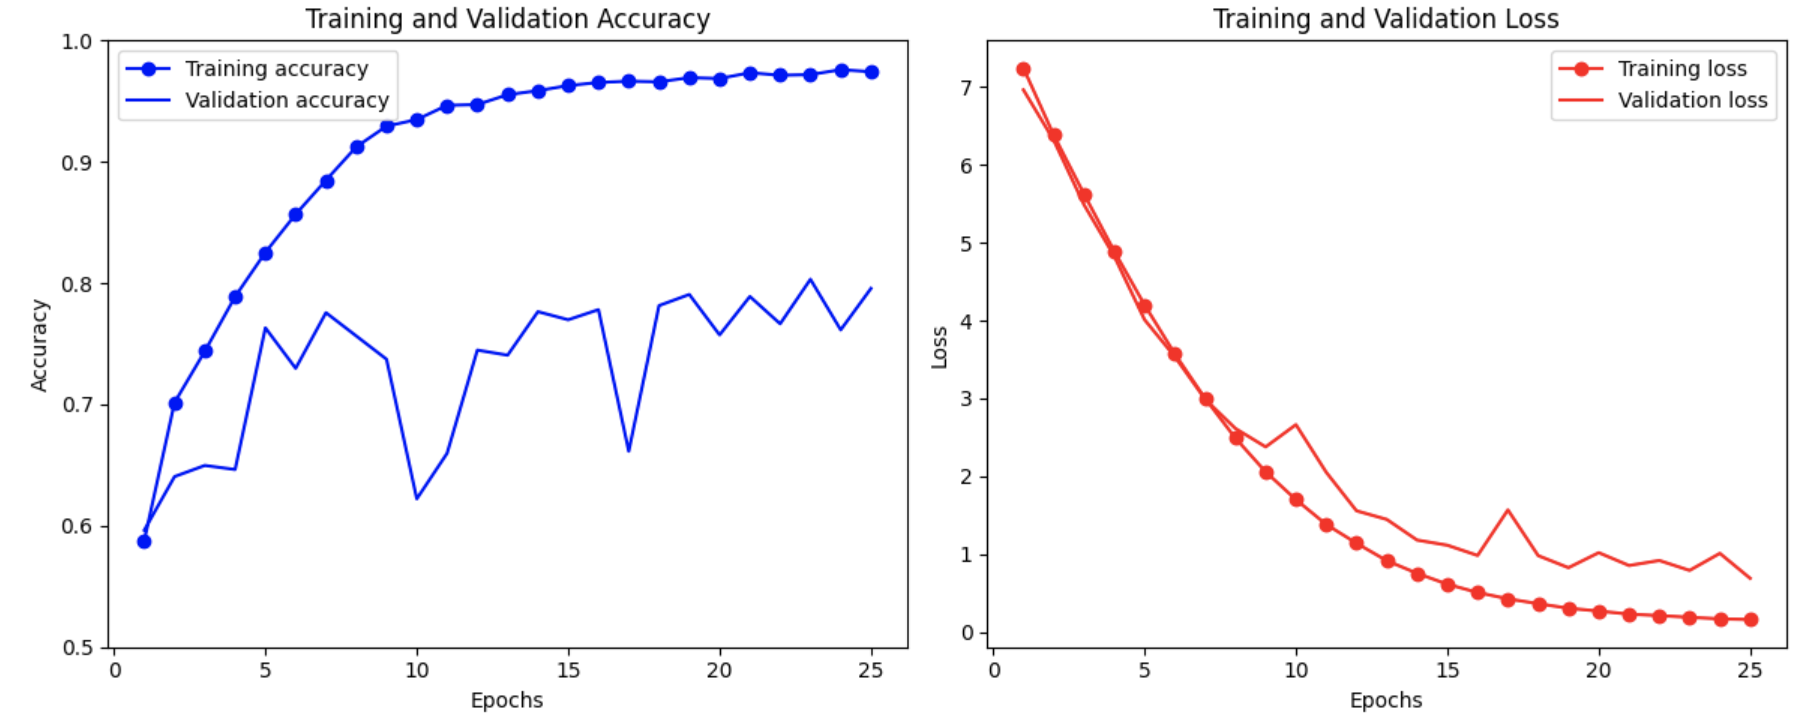
\includegraphics[width=0.75\linewidth]{learningCurves.png}
    \caption{Learning curve of our model.}
    \label{fig:fig4}
\end{figure}



%% TODO: write about what you conclude. This is not meant to be a summary section but more of a takeaways/future work section.
%% Must contain:
%% - Any concrete takeaways or conclusions from your experiments/results/project
%%
%% You can also discuss limitations here if you want.
%%
\section{Conclusions}

% TODO:

One limitation of our project is that deepfake images which appear online are generated by a significantly higher number of models and machine learning techniques than the three used to train our model. Including a wider variety of image generation methods in our data would make our model a better solution to the problem we attempted to solve by making it more effective at accurately classifying the deepfakes that internet users encounter online.

One way our model's accuracy could be improved in future work is by performing data augmentation on the existing images in the dataset to obtain more data with slightly different features. In both the real and deepfake images in DeepFakeFace, faces appear at various distances and angles, so our initial attempts at data augmentation would consist of rotating and cropping images, though other methods, such as translating or adjusting image brightness, may also be effective.

We observed notable improvements in our model's performance as the volume of training data increased. However, to keep the training time manageable, we had to limit the amount of data used. It is likely that utilizing the entire dataset would yield even better results, further surpassing our initial performance benchmarks. Despite these limitations, we were still able to achieve significantly better results than the baseline comparisons. 


%%%%

\bibliography{refs}
\bibliographystyle{plain}


\end{document} % end tag of the document
